\documentclass[
  11pt,
  letterpaper,
   addpoints,
  % answers
  ]{exam}

\usepackage{../exercise-preamble}
\usepackage{multicol}
\begin{document}

\noindent
\begin{minipage}{0.47\textwidth}

\includegraphics[width=\textwidth]{../fcfm_die}
\end{minipage}
\begin{minipage}{0.53\textwidth}
    
\begin{center} 
\large\textbf{Análisis y Diseño de Circuitos Eléctricos} (EL3101-2) \\
\large\textbf{Tarea 1} \\
\normalsize Prof.~Santiago Bradford V.\\
\normalsize Prof.~Aux.~Erik Saez A. - Rodrigo Catalán\\
             - Byron Castro R.
\end{center}
\end{minipage}

\vspace{0.5cm}
\noindent
\vspace{.85cm}

\fbox{%
  \begin{minipage}{0.95\linewidth}
    \textbf{Obs:} Recuerde que solo serán revisadas tres preguntas al azar. No olvide explicar de forma clara y precisa su desarrollo. \\\\
    \textbf{Fecha de entrega}: Domingo 27 de Abril
  \end{minipage}
}

\begin{questions}
    %%%%%%%%%%%%%%%%%%%%%%%%%%%%
    \question     
    Para el circuito de la figura (donde solo los puntos son nodos), calcular:
    \begin{enumerate}
        \item La corriente $I_f$
        \item La diferencia de potencial entre los nodos A y B
        \item La diferencia de potencial entre los nodos C y D
        \item La caída de tensión $V_2$
        \begin{center}
            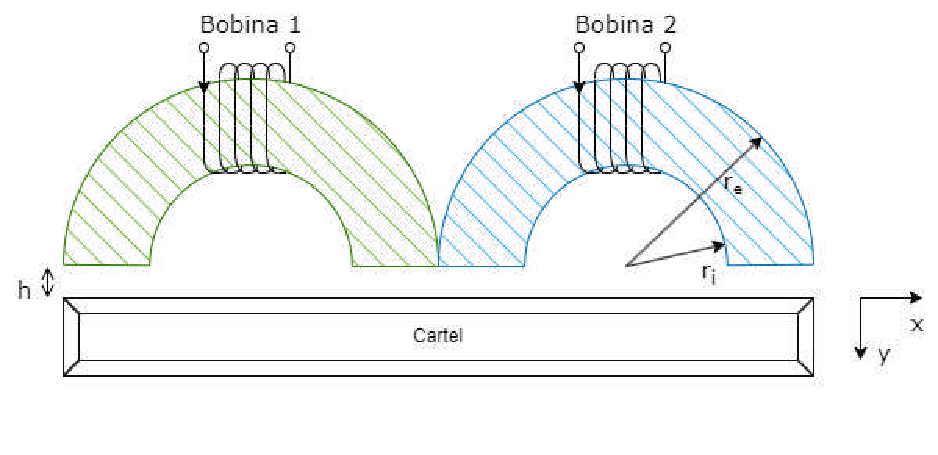
\includegraphics[width=0.35\textwidth]{Tarea_1_1}
            \captionof{figure}{Esquema del problema}
        \end{center}
    \end{enumerate}
    %%%%%%%%%%%%%%%%%%%%%%%%%%%%
    \begin{solution}
        a
    \end{solution}
    %%%%%%%%%%%%%%%%%%%%%%%%%%%
    \question  Encontrar el voltaje de salida $v_O$ en función de los valores de las resistencias y del parámetro $\beta$ en el circuito.
    \begin{center}
        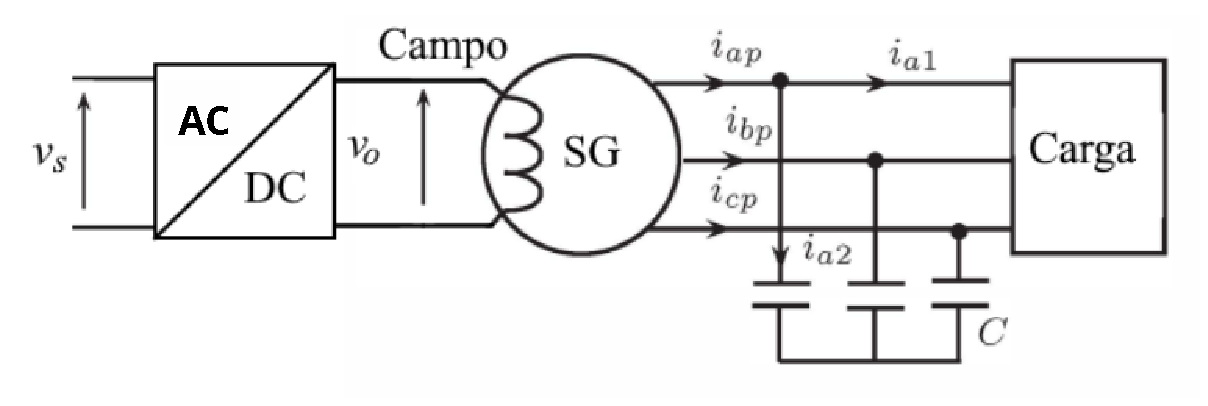
\includegraphics[width=0.55\textwidth]{Tarea_1_2}
        \captionof{figure}{Esquema del circuito}
    \end{center}
    %%%%%%%%%%%%%%%%%%%%%%%%%%%
    \begin{solution}
       a
    \end{solution}
%%%%%%%%%%%%%%%%%%%%%%%%%%%
\question  Para el circuito de diodos ideales de la figura mostrada. Nota: En las partes a) y b) se recomienda primero redibujar el circuito y determinar $V^+$, $V^-$, $i_+$ y $i_-$ en el OPAMP de la salida B.

\begin{enumerate}
    \item[a)] Para el caso D1 ON, D2 OFF encuentre $V_{0A}$ y $V_{0B}$, y la condición sobre $V_i$ para que los diodos operen en estos estados.

    \item[b)] Para el caso D1 OFF, D2 ON encuentre $V_{0A}$ y $V_{0B}$, y la condición sobre $V_i$ para que los diodos operen en estos estados.

    \item[c)] Si la entrada es $V_i = A \cdot \sin(\omega t)$, dibuje la salida $V_{0B}$ en función del tiempo a partir de los resultados obtenidos en a) y b). ¿Cuál es la función de este circuito?
\end{enumerate}
\begin{center}
    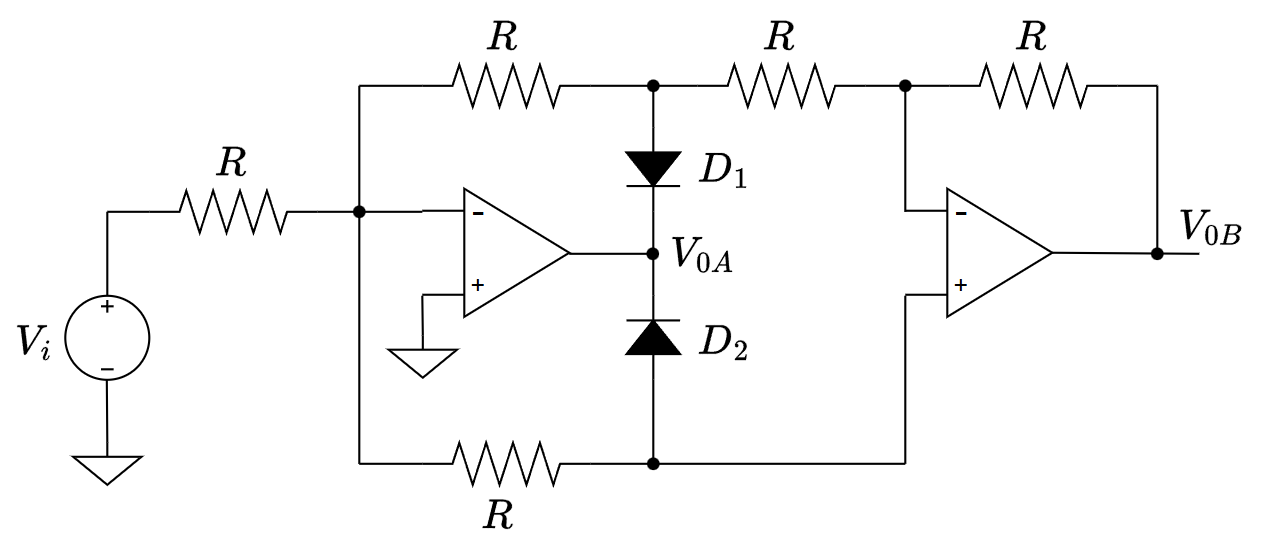
\includegraphics[width=0.6\textwidth]{Tarea_1_3}
    \captionof{figure}{Esquema del circuito}
\end{center}
%%%%%%%%%%%%%%%%%%%%%%%%%%%
\begin{solution}
    a
\end{solution}
%%%%%%%%%%%%%%%%%%%%%%%%%%%
\question Considere el circuito de la figura. Notar que está compuesto por Opamps que usted debe considerar como ideales. Bajo las propiedades de Opamps ideales, calcule el voltaje en todos los nodos (excepto el de tierra)
\begin{center}
    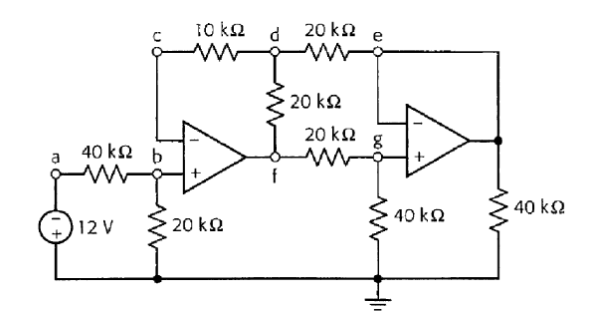
\includegraphics[width=0.5\textwidth]{Tarea_1_6}
    \captionof{figure}{Esquema del circuito}
\end{center}
%%%%%%%%%%%%%%%%%%%%%%%%%%%%%
\newpage
\question Para el circuito de la figura, los diodos $D1$ y $D2$ \textbf{no son ideales}
\begin{center}
    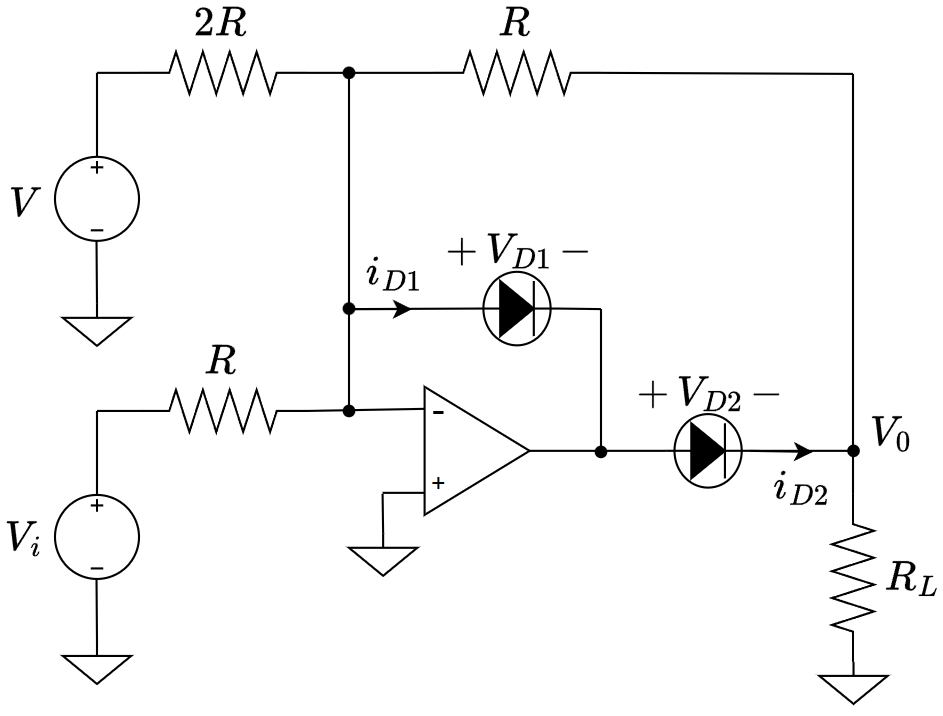
\includegraphics[width=0.4\textwidth]{Tarea_1_4}
    \captionof{figure}{Esquema del circuito}
\end{center}
\begin{enumerate}
    \item Plantee las ecuaciones nodales que relacionan $i_{D1}$ e $i_{D2}$ con las fuentes y parámetros del circuito. Plantee una ecuación de LVK que incluya $V_{D1}$ y $V_{D2}$.
    \item Reemplace los diodos no ideales por un modelo que incluye un diodo ideal en serie con una fuente de voltaje $V_T>0$ como se muestra en la figura a continuación. Modifique las ecuaciones del ítem anterior para incluir este cambio ($V_T\ll V_i$ y $V_T\ll V$).
    \begin{center}
        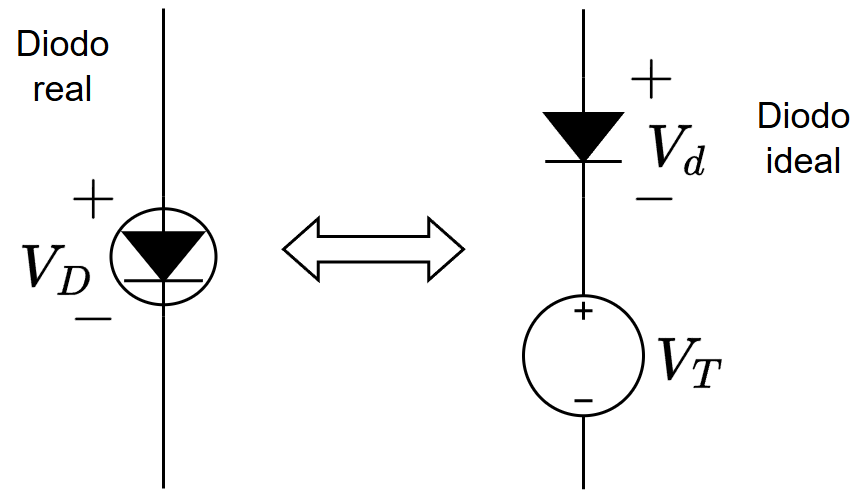
\includegraphics[width=0.3\textwidth]{Tarea_1_5}
        \captionof{figure}{Esquema del circuito}
    \end{center}
    Si D1 ON y D2 OFF, dibuje el circuito resultante cuando se incluye el modelo del diodo
    real. Apóyese en él y las ecuaciones para encontrar el voltaje de salida del OPAMP y el voltaje $V_{d2}$ en el diodo ideal.
    
    \item Analice matemáticamente los casos (D1 ON, D2 OFF) y (D1 OFF, D2 ON). Encuentre restricciones sobre la fuente $V_i$ y determine el voltaje de salida $V_0$ del circuito.
\end{enumerate}
%%%%%%%%%%%%%%%%%%%%%%%%%%%
\begin{solution}
   A
\end{solution}
%%%%%%%%%%%%%%%%%%%%%%%%%%%

\newpage
\question Para el circuito de la figura, observe que el interruptor es controlado por un voltaje externo al circuito presentado. Ante ello, se busca obtener un rango de valores posibles de $R_D$ que pueda cumplir con los siguientes requisitos de diseño:

\begin{enumerate}
    \item Si el interruptor está abierto (conectado a $R_{OFF}$), entonces, $V_0 > 3{,}5\,\mathrm{[V]}$
    \item Si el interruptor está cerrado (conectado a $R_{ON}$), entonces, $V_0 < 0{,}5\,\mathrm{[V]}$
    \item La corriente máxima que pasa por el interruptor debe ser $1\,\mathrm{[mA]}$
    \item La fuente debe entregar una potencia máxima $< 25\,\mathrm{[mW]}$
\end{enumerate}
\begin{center}
    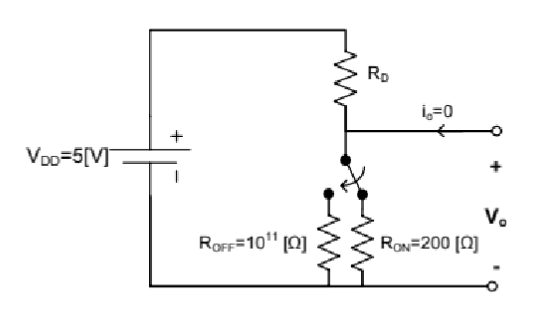
\includegraphics[width=0.5\textwidth]{Tarea_1_7}
    \captionof{figure}{Esquema del circuito}
\end{center}
\end{questions}
\end{document}